% !BIB TS-program = biber

\RequirePackage[l2tabu,orthodox]{nag}

% TODO: decide if one-sided/two-sided
%\documentclass[headsepline,footsepline,footinclude=false,fontsize=11pt,paper=a4,listof=totoc,bibliography=totoc,BCOR=12mm,DIV=12]{scrbook} % two-sided
\documentclass[headsepline,footsepline,footinclude=false,oneside,fontsize=11pt,paper=a4,listof=totoc,bibliography=totoc]{scrbook} % one-sided

% TODO: change citation style in settings
\PassOptionsToPackage{table,svgnames,dvipsnames}{xcolor}

\usepackage[utf8]{inputenc}
\usepackage[T1]{fontenc}
\usepackage[sc]{mathpazo}
\usepackage[ngerman,american]{babel}
\usepackage[autostyle]{csquotes}
\usepackage[%
  backend=biber,
  url=true,
  style=alphabetic,
  maxnames=4,
  minnames=3,
  maxbibnames=99,
  giveninits,
  uniquename=init]{biblatex} % TODO: adapt citation style
\usepackage{graphicx}
\usepackage{scrhack} % necessary for listings package
\usepackage{listings}
\usepackage{lstautogobble}
\usepackage{tikz}
\usepackage{pgfplots}
\usepackage{pgfplotstable}
\usepackage{booktabs}
\usepackage[final]{microtype}
\usepackage{caption}
\usepackage[printonlyused]{acronym}
\usepackage[hidelinks]{hyperref} % hidelinks removes colored boxes around references and links
\AtBeginDocument{%
	\hypersetup{
		pdftitle=\getTitle,
		pdfauthor=\getAuthor,
	}
}
\usepackage{ifthen}

\addto\extrasamerican{
	\def\lstnumberautorefname{Line}
	\def\chapterautorefname{Chapter}
	\def\sectionautorefname{Section}
	\def\subsectionautorefname{Subsection}
	\def\subsubsectionautorefname{Subsubsection}
}

\addto\extrasngerman{
	\def\lstnumberautorefname{Zeile}
}

% Themes
\ifthenelse{\equal{\detokenize{dark}}{\jobname}}{%
  % Dark theme
  \newcommand{\bg}{black} % background
  \newcommand{\fg}{white} % foreground
  \usepackage[pagecolor=\bg]{pagecolor}
  \color{\fg}
}{%
  % Light theme
  \newcommand{\bg}{white} % background
  \newcommand{\fg}{black} % foreground
}

\bibliography{bibliography}

\setkomafont{disposition}{\normalfont\bfseries} % use serif font for headings
\linespread{1.05} % adjust line spread for mathpazo font

% Add table of contents to PDF bookmarks
\BeforeTOCHead[toc]{{\cleardoublepage\pdfbookmark[0]{\contentsname}{toc}}}

% Define TUM corporate design colors
% Taken from http://portal.mytum.de/corporatedesign/index_print/vorlagen/index_farben
\definecolor{TUMBlue}{HTML}{0065BD}
\definecolor{TUMSecondaryBlue}{HTML}{005293}
\definecolor{TUMSecondaryBlue2}{HTML}{003359}
\definecolor{TUMBlack}{HTML}{000000}
\definecolor{TUMWhite}{HTML}{FFFFFF}
\definecolor{TUMDarkGray}{HTML}{333333}
\definecolor{TUMGray}{HTML}{808080}
\definecolor{TUMLightGray}{HTML}{CCCCC6}
\definecolor{TUMAccentGray}{HTML}{DAD7CB}
\definecolor{TUMAccentOrange}{HTML}{E37222}
\definecolor{TUMAccentGreen}{HTML}{A2AD00}
\definecolor{TUMAccentLightBlue}{HTML}{98C6EA}
\definecolor{TUMAccentBlue}{HTML}{64A0C8}

% Settings for pgfplots
\pgfplotsset{compat=newest}
\pgfplotsset{
  % For available color names, see http://www.latextemplates.com/svgnames-colors
  cycle list={TUMBlue\\TUMAccentOrange\\TUMAccentGreen\\TUMSecondaryBlue2\\TUMDarkGray\\},
}

% Settings for lstlistings
\lstset{%
  basicstyle=\ttfamily,
  columns=fullflexible,
  autogobble,
  keywordstyle=\bfseries\color{TUMBlue},
  stringstyle=\color{TUMAccentGreen},
  captionpos=b
}


% TODO: change thesis information
\newcommand*{\getUniversity}{Technische Universität München}
\newcommand*{\getFaculty}{Computational Science and Engineering}
\newcommand*{\getSchool}{Computation, Information and Technology}
\newcommand*{\getTitle}{Wave Reversal in SeisSol using the Instantaneous Time Mirror}
\newcommand*{\getTitleGer}{Wellenumkehr in SeisSol unter Verwendung des Instantaneous Time Mirror}
\newcommand*{\getAuthor}{Vikas Kurapati}
\newcommand*{\getDoctype}{Master's Thesis}
\newcommand*{\getSupervisor}{Prof. Dr. Michael Bader}
\newcommand*{\getAdvisor}{M.Sc. Lukas Krenz, M.Sc. Sebastian Wolf}
\newcommand*{\getSubmissionDate}{October 15, 2023}
\newcommand*{\getSubmissionLocation}{Garching bei München}

\usepackage{amsmath}
\usepackage{mathtools}
\usepackage{textgreek}
\usepackage{graphicx}

\begin{document}

% Set page numbering to avoid "destination with the same identifier has been already used" warning for cover page.
% (see https://en.wikibooks.org/wiki/LaTeX/Hyperlinks#Problems_with_Links_and_Pages).
\pagenumbering{alph}
\begin{titlepage}
  % HACK for two-sided documents: ignore binding correction for cover page.
  % Adapted from Markus Kohm's KOMA-Script titlepage=firstiscover handling.
  % See http://mirrors.ctan.org/macros/latex/contrib/koma-script/scrkernel-title.dtx,
  % \maketitle macro.
  \oddsidemargin=\evensidemargin\relax
  \textwidth=\dimexpr\paperwidth-2\evensidemargin-2in\relax
  \hsize=\textwidth\relax

  \centering

  \IfFileExists{logos/tum-\fg.pdf}{%
    \includegraphics[height=20mm]{logos/tum-\fg.pdf}
  }{%
    \vspace*{20mm}
  }

  \vspace{5mm}
  {\huge\MakeUppercase{School of \getSchool{}} \par}

  \vspace{5mm}
  {\large\MakeUppercase{\getUniversity{}} \par}

  \vspace{15mm}
  {\Large \getDoctype{} in \getChair{} \par}

  \vspace{10mm}
  {\huge\bfseries \getTitle{} \par}

  \vspace{10mm}
  {\LARGE \getAuthor{}}

  \IfFileExists{logos/faculty-\fg.pdf}{%
    \vfill{}
    \includegraphics[height=20mm]{logos/faculty-\fg.pdf}
  }{}
\end{titlepage}


\frontmatter{}

\begin{titlepage}
  \centering

  \IfFileExists{logos/tum-\fg.pdf}{%
    \includegraphics[height=20mm]{logos/tum-\fg.pdf}
  }{%
    \vspace*{20mm}
  }

  \vspace{5mm}
  {\huge\MakeUppercase{School of \getSchool{}} \par}

  \vspace{5mm}
  {\large\MakeUppercase{\getUniversity{}} \par}

  \vspace{20mm}
  {\Large \getDoctype{} in \getChair{} \par}

  \vspace{15mm}
  {\huge\bfseries \getTitle{} \par}

%  \vspace{7.5mm}
%  {\huge\bfseries \foreignlanguage{ngerman}{\getTitleGer{}} \par}

  \vspace{15mm}
  \begin{tabular}{l l}
    Author:          & \getAuthor{}         \\
    Supervisor:      & \getSupervisor{}     \\
    Advisor:         & \getAdvisor{}        \\
    Submission Date: & \getSubmissionDate{} \\
  \end{tabular}

  \IfFileExists{logos/faculty-\fg.pdf}{%
    \vfill{}
    \includegraphics[height=20mm]{logos/faculty-\fg.pdf}
  }{}
\end{titlepage}

\thispagestyle{empty}
\vspace*{0.8\textheight}
\noindent
I confirm that this \MakeLowercase{\getDoctype{}} is my own work and I have documented all sources and material used.

\vspace{15mm}
\noindent
\getSubmissionLocation{}, \getSubmissionDate{} \hspace{50mm} \getAuthor{}

\cleardoublepage{}

\addcontentsline{toc}{chapter}{Acknowledgments}
\thispagestyle{empty}

\vspace*{20mm}

\begin{center}
    {\usekomafont{sectioning}\usekomafont{section} Acknowledgments}
\end{center}

\vspace{10mm}

%TODO: Acknowledgments
I would like to express my deepest gratitude to my supervisor, Prof. Dr. Michael Bader and my advisor, Lukas Krenz 
for their invaluable guidance, support, and encouragement throughout my master's thesis. 
Their vast knowledge, constructive criticism, and prompt feedback helped shape my ideas and made this thesis possible. \\

I would like to thank Prof. Gregor Hillers for giving me the opportunity and welcoming me to Helsinki, Finland to collaborate with the team at University of Helsinki
to work and get more ideas to work on my thesis. I would also like to thank Prof. Alice Gabriel for being involved in the project and providing us valuable inputs.
The discussions have helped me get ideas on how to go about the thesis and the project in general.\\

I would also like to thank the faculty members of the Chair of Scientific Computing for their continuous support and for providing 
me with a challenging yet rewarding academic experience. Their passion and dedication to teaching and research have been a 
great source of inspiration to me. \\

I am indebted to my family and friends for their unwavering support, encouragement, and patience during this challenging 
journey. Their love and faith in me have been my constant motivation. \\

\cleardoublepage{}

\chapter{\abstractname}

%TODO: Abstract

\microtypesetup{protrusion=false}
\tableofcontents{}
\microtypesetup{protrusion=true}

\mainmatter{}

% !TeX root = ../main.tex
% Add the above to each chapter to make compiling the PDF easier in some editors.

\chapter{Introduction}\label{chapter:introduction}

Studying seismic phenomena provides valuable insights and potential techniques for identifying areas that more susceptible to earthquakes, mitigating economic impacts, 
and reducing casualities. \\

The field of earthquake simulation has seen significant advancements in recent years, thanks to the availability of powerful supercomputers ~\parencite{inproceedings}, ~\parencite{breuer}, ~\parencite{seissol}.
With these resources, it has become possible to model realistic 3D earthquake events on a large scale, something that was not feasible until a few decades ago. 
Todays simulation software relies heavily on numerical methods to approximate real life physics. In this process, the volume of the problem is discretized into smaller elements, and numerical solvers are employed in each element to obstain a solution.
A few examples out of these wide range of numerical methods used to solve wave equations are finite differences, finite volumes, finite elements. These numerical methods have played a crucial role in advancing the field of earthquake simulation and are continuously being improved to produce more accurate and efficient simulations. \\

SeisSol~\footnote{\href{https://seissol.org}{https://seissol.org}} is a scientific software that enables the simulation of seismic waves and earthquake phenomena. 
However, modeling complex 3D geometries is computationally intensive for modeling complex 3D geometries.
To address this challenge, SeisSol implements an efficient way to optimally utilize the computing resources. 
The software allows for the study of various scenarios, including adjusting material properties to exhibit elastic, viscoelastic and viscoplastic behaviour.
SeisSol utilizes a combination of \ac{DG} method and \ac{ADER} time-integration approach to solve the problems.
This combination is called \ac{ADER}-\ac{DG} approach ~\parencite{dumbser}. Dumbser et al. extended this approach to solve the elastic wave equations in three dimensions ~\parencite{dumbser1}. The \ac{ADER}-\ac{DG} approach provides arbitrary high-order accuracy in space and time, with the solution in each element approximated by polynomials.
The degrees of freedom are expressed through the coefficients of the polynomial, which are advanced in time during simulation, allowing for discontinuities across element boundaries ~\parencite{martin}. \\

In this thesis, we extend SeisSol with the implementation of Wave Reversal of Seismic waves using the \acf{ITM}. 
Time-reversal techniques have been researched in the field of acoustic media, primarily in order to focus the wave below
the diffraction limit ~\parencite{67072}. This methodology may be applied, for instance, to improve the detection of gallstones within the human body ~\parencite{10.1063/1.881692}. 
In the context of seismic waves, time-reversal methods may be employed to investigate the source and origin of the seismic waves.
The work by ~\parencite{Fink2017} describes two techniques for wave reversal, the time-reversal mirror approach and the instantaneous time mirror 
mimicking Loschmidt~\footnote{\href{https://en.wikipedia.org/wiki/Loschmidt\%27s_paradox}{Loschmidt's Paradox}}~\parencite{wu1975}, ~\parencite{binder2023}, ~\parencite{loschmidt} point of view
 for waves. 
While both techniques generate time-reversed waves, we specifically focus on the second approach. 
This method involves manipulating waves on time boundaries by sudden modifications of the wave properties like wave speed in the whole medium, 
effectively mimicking the Loschmidt point of view. 
This approach is very efficient for radiating time-reversed waves without the use of any antennas or receivers. 
The first approach, which utilizes "time-reversal mirrors" with wave manipulation along a spatial boundary sampled by a finite number of antennas, has numerous applications in telecommunication, imaging, therapy, and defense ~\parencite{Fink2017}. 
~\parencite{Bacot2016} have experimentally demonstrated the instantaneous time mirrors on surface waves on water by manipulating the wave speed for a period of time using a vertical jolt.
This is shown to refocus the waves at the source position before diverging again.\\

To achieve \ac{ITM}s in a simulation environment, we modify the velocities of waves for a short period of time $t_{ITM}$ to $t_{ITM} + \tau$ by manipulating 
the material properties $\lambda, \mu, \rho$. As the velocities of waves depend on these three properties, this manipulation is 
sufficient to modify wave velocities and achieve wave reversal using \ac{ITM}s.

It is important to note that the time-reversal presented here, in its simplest form, may not be directly useful in experimental 
investigations, as we cannot directly modify the material properties. However, it does provide an approach to approximately 
locate the source of an earthquake when successfully reversed. \\

The thesis is organized as follows: Chapter \ref{chapter:seismicwaves} focuses on the fundamental theory of elastic wave propagation and the presentation
of the numerical \ac{ADER}-\ac{DG} scheme as used in SeisSol. The equation of motion in elastic media is derived, and the wave equation is presented
in the velocity-stress formulation. Chapter \ref{chapter:TimeReversal} outlines the theory of time-reversal, briefly discussing the wave reversal approach before
delving into a more detailed explanation of the \ac{ITM}s concept. Section \ref{section:Implementation} describes the method and implementation details of \ac{ITM}s
in SeisSol. Chapter \ref{chapter:Results} discusses the different parametric studies and results obtained in the process. Finally, we discuss the results
and possible future research directions in Chapter \ref{chapter:Conclusion}. 

%See~\autoref{tab:sample}, \autoref{fig:sample-drawing}, \autoref{fig:sample-plot}, \autoref{fig:sample-listing}.
% 
% \begin{table}[htpb]
%   \caption[Example table]{An example for a simple table.}\label{tab:sample}
%   \centering
%   \begin{tabular}{l l l l}
%     \toprule
%       A & B & C & D \\
%     \midrule
%       1 & 2 & 1 & 2 \\
%       2 & 3 & 2 & 3 \\
%     \bottomrule
%   \end{tabular}
% \end{table}
% 
% \begin{figure}[htpb]
%   \centering
%   % This should probably go into a file in figures/
%   \begin{tikzpicture}[node distance=3cm]
%     \node (R0) {$R_1$};
%     \node (R1) [right of=R0] {$R_2$};
%     \node (R2) [below of=R1] {$R_4$};
%     \node (R3) [below of=R0] {$R_3$};
%     \node (R4) [right of=R1] {$R_5$};
% 
%     \path[every node]
%       (R0) edge (R1)
%       (R0) edge (R3)
%       (R3) edge (R2)
%       (R2) edge (R1)
%       (R1) edge (R4);
%   \end{tikzpicture}
%   \caption[Example drawing]{An example for a simple drawing.}\label{fig:sample-drawing}
% \end{figure}
% 
% \begin{figure}[htpb]
%   \centering
% 
%   \pgfplotstableset{col sep=&, row sep=\\}
%   % This should probably go into a file in data/
%   \pgfplotstableread{
%     a & b    \\
%     1 & 1000 \\
%     2 & 1500 \\
%     3 & 1600 \\
%   }\exampleA
%   \pgfplotstableread{
%     a & b    \\
%     1 & 1200 \\
%     2 & 800 \\
%     3 & 1400 \\
%   }\exampleB
%   % This should probably go into a file in figures/
%   \begin{tikzpicture}
%     \begin{axis}[
%         ymin=0,
%         legend style={legend pos=south east},
%         grid,
%         thick,
%         ylabel=Y,
%         xlabel=X
%       ]
%       \addplot table[x=a, y=b]{\exampleA};
%       \addlegendentry{Example A};
%       \addplot table[x=a, y=b]{\exampleB};
%       \addlegendentry{Example B};
%     \end{axis}
%   \end{tikzpicture}
%   \caption[Example plot]{An example for a simple plot.}\label{fig:sample-plot}
% \end{figure}
% 
% \begin{figure}[htpb]
%   \centering
%   \begin{tabular}{c}
%   \begin{lstlisting}[language=SQL]
%     SELECT * FROM tbl WHERE tbl.str = "str"
%   \end{lstlisting}
%   \end{tabular}
%   \caption[Example listing]{An example for a source code listing.}\label{fig:sample-listing}
% \end{figure}
% 
% !TeX root = ../main.tex
% Add the above to each chapter to make compiling the PDF easier in some editors.

\chapter{Seismic Waves and ADER-DG formulation}\label{chapter:seismicwaves}
In this chapter, the necessary theoretical foundations for this thesis are established through the derivation of fundamental equations governing the propagation of elastic waves.
The equation of motion corresponding to this will be presented later on in the velocity-stress formulation.
We only consider isotropic media and utilize this assumption in particular symmtery arguments. The restriction to isotropic media is a commonly employed simplification, as seen in works such as ~\parencite{dumbser1}.

The section \ref{section:ADER-DG} discusses the fundamental framework of SeisSol, the numerical tool employed for simulating seismic wave phenomena. SeisSol is a combination
of the \ac{DG-FE} method and a time integration scheme based on the solution of \ac{ADER}, as described in previous works ~\parencite{dumbser1}, ~\parencite{seissol}. This approach, known as 
\ac{ADER}-\ac{DG} will be introduced in more detail.

\section{Elastic Wave Equation}\label{section:elasticwaveequation}
An elastic medium is characterized by an undeformed state, in which stresses and strains are zero, to which it will return to in the absence
of outer forces. If the stresses and strains the medium experiences are infinitesimal, the theory of linear elasticity applies. We define
the displacement vector, $\mathbf{U}$, describing the shortest distance between the initial and current position of a point. The particle
velocities $u,v$ and $w$ in $x, y$ and $z$ direction, respectively, can then be defined as the temporal derivative of $\mathbf{U}$
\begin{align}
    \begin{split}
    \frac{\partial U_x}{\partial t} &= \dot{U}_x = u, \\
    \frac{\partial U_y}{\partial t} &= \dot{U}_y = v, \\
    \frac{\partial U_z}{\partial t} &= \dot{U}_z = w, \\
    \end{split}
 \end{align}
where the subscript denotes the coordinate direction and a dot over a variable represents its partial time derivative leading to the following notation:
\begin{align}
    \begin{split}
        \frac{\partial U_i}{\partial t} = \dot{U}_i = V_i,
    \end{split}
    \label{equation1}
\end{align}
where the velocity vector, $\mathbf{V}$, is introduced for convenience. $\mathbf{V} = [V_1, V_2, V_3] = [u, v ,w]$ are used analogously.\\

In the context of linear elasticity, the following extension of Hooke's law  to generalize linear elasticity holds
\begin{align}
    \begin{split}
        \sigma_{ij} = c_{ijkl}\epsilon_{kl},
    \end{split}
    \label{eq:hookeslaw}
\end{align}
with the medium specific constants $c_{ijkl}$. The Einstein summation convention
is followed, where an index appearing twice is summed over all possible values. In this context, $\sigma_{ij}$ represents the stress tensor
and $\epsilon_{kl}$ represents the strain tensor. Hooke's law expresses that stress tensor components are linear combinations of strain tensor
components. For infinitesimally small perturbations, the strain tensor components $\epsilon_{kl}$ are defined as follows
\begin{align}
    \begin{split}
        \epsilon_{kl} = \frac{1}{2}\left(\partial_k U_l + \partial_l U_k \right) ,
    \end{split}
\end{align}
where $\partial_k$ represents the spatial derivative in $k$-direction and $U_i$ represents the displacement in $i$-direction.
Previously, we mentioned our focus on the velocity-stress formulation rather than the displacement-stress formulation.
To eliminate the displacements $U_i$, we introduced velocities $V_i$ in equation \ref{equation1}.
Consequently, this leads to the time derivative of the strain tensor
\begin{align}
    \begin{split}
        \partial_t \epsilon_{kl} = \frac{1}{2}\left(\partial_k V_l + \partial_l V_k \right) ,
        % \dot{\epsilon}_{kl} = \frac{1}{2}\left( \partial_k V_l + \partial_l V_k \right) ,
    \end{split}
\end{align}
expressed in terms of the spatial derivatives of the velocities $V_i$. Here, $\partial_t$ denotes the time derivative. As the constants $c_{ijkl}$ remain constant over time,
\begin{align}
    \begin{split}
        \partial_t \sigma_{ij} = c_{ijkl} \partial_t {\epsilon}_{kl} .
    \end{split}
    \label{eq:stress}
\end{align}

We can apply symmetry considerations of the stress tensor i.e., $\sigma_{ij} = \sigma_{ji}$ to the term $c_{ijkl}$ in equation \ref{eq:hookeslaw} and reduce the number of independent components from 81 to 21 ~\parencite[Cha. 2]{aki2002quantitative}.
This in turn lets us define the tensor in terms of two constants in isotropic media with the general form of
\begin{equation}
    c_{ijkl} = \lambda \delta_{ij}\delta_{kl} + \mu\left(\delta_{ik}\delta_{jl} + \delta_{il}\delta_{jk}\right),
    \label{eq:isotropic}
\end{equation}
where $\delta$ is the Kronecker delta function and $\lambda, \mu$ are the Lam\'e parameters. \\

We now write a force balance in a volume $V$ within a surface $S$. The momentum within the volume changes at a rate equal
to the forces acting on that volume. Therefore, the forces acting on these comprise a body force and a surface force, which result
from the presence of normal and shear stresses. This can be written mathematically as 

\begin{equation}
    \frac{\partial}{\partial t} \int_V \rho \frac{\partial \mathbf{U}}{\partial t}dV = \int_V \mathbf{f}dV + \oint_S \mathbf{T\left(n\right)}dS,
    \label{eq:forcebalance}
\end{equation}
where $\frac{\partial}{\partial t} \int_V \rho \frac{\partial \mathbf{U}}{\partial t}dV$, is the momentum of the control volume with density $\rho$, and $\mathbf{T}$
is the traction vector which is related to the stress tensor by Cauchy's stress theorem %~\parencite{cauchy-stress-theorem}
\begin{equation}
    T_j\left(n\right) = \sigma_{ij}n_i,
    \label{eq:tractionvector}
\end{equation}
with the normal vector $n_i$. Applying Gauss' divergence theorem

\begin{equation}
    \oint_S \mathbf{T\left(n\right)}dS = \oint_S \sigma_{ij}n_idS = \int_V \partial_j \sigma_{ij}dV,
\label{eq:gaussdivergence}
\end{equation}

Replacing $\mathbf{T}$ in equation \refeq{eq:forcebalance} using equations \ref{eq:tractionvector} and \ref{eq:gaussdivergence} and reordering the terms gives us

\begin{equation}
    \int_V \left(\rho \frac{\partial^2 {U}_i}{\partial t^2} - f_i - \partial_j \sigma_{ij}\right)dV = 0.
\end{equation}

Here we assumed that the stress tensor is symmetric, i.e., $\sigma_{ij}=\sigma_{ji}$. As it is true for any general volume, we can
equate the integrand to zero. This gives us the equation
\begin{equation}
    \rho \frac{\partial^2 {U}_i}{\partial t^2} = f_i + \partial_j \sigma_{ij}.
    \label{eq:force}
\end{equation}

Expanding equation \ref{eq:force} in $j$ and using $V_i = \frac{\partial U_i}{\partial t}$, we get
\begin{equation}
    \rho \frac{\partial V_i}{\partial t} = f_i + \partial_x \sigma_{xi} + \partial_y \sigma_{yi} + \partial_z \sigma_{zi},
    \label{eq:finalequation}
\end{equation}

The body force $f_i$ will be discussed later in terms of the source terms. \\
\par Combining equations \ref{eq:stress}, \ref{eq:isotropic} and \ref{eq:finalequation}, we obtain the final 3D 
wave elastic equation for an isotropic medium in velocity-stress formulation as follows
\begin{align}
    \begin{split}
    \frac{\partial \sigma_{xx}}{\partial t} - \left(\lambda  + 2\mu\right)\frac{\partial u}{\partial x} - \lambda \frac{\partial v}{\partial y} - \lambda\frac{\partial w}{\partial z} &= S_1, \\    
    \frac{\partial \sigma_{yy}}{\partial t} - \lambda \frac{\partial u}{\partial x} - \left( \lambda + 2 \mu \right)\frac{\partial v}{\partial y} - \lambda \frac{\partial w}{\partial w} &= S_2, \\
    \frac{\partial \sigma_{zz}}{\partial t} - \lambda \frac{\partial u}{\partial x} - \lambda \frac{\partial v}{\partial y} - \left(\lambda + 2\mu\right)\frac{\partial w}{\partial z} &= S_3, \\
    \frac{\partial \sigma_{xy}}{\partial t} - \mu \left(\frac{\partial v}{\partial x} + \frac{\partial u}{\partial y}\right) &= S_4, \\ 
    \frac{\partial \sigma_{yz}}{\partial t} - \mu \left(\frac{\partial v}{\partial z} + \frac{\partial w}{\partial y}\right) &= S_5, \\
    \frac{\partial \sigma_{xz}}{\partial t} - \mu \left(\frac{\partial u}{\partial z} + \frac{\partial w}{\partial x}\right) &= S_6, \\
    \rho \frac{\partial u}{\partial t} - \frac{\partial \sigma_{xx}}{\partial x} - \frac{\partial \sigma_{xy}}{\partial y} - \frac{\partial \sigma_{xz}}{\partial z} &= \rho S_7, \\
    \rho \frac{\partial v}{\partial t} - \frac{\partial \sigma_{xy}}{\partial x} - \frac{\partial \sigma_{yy}}{\partial y} - \frac{\partial \sigma_{yz}}{\partial z} &= \rho S_8, \\
    \rho \frac{\partial w}{\partial t} - \frac{\partial \sigma_{xz}}{\partial x} - \frac{\partial \sigma_{yz}}{\partial y} - \frac{\partial \sigma_{zz}}{\partial z} &= \rho S_9, \\
\end{split}
\label{eq:setofequations}
\end{align}
where $S_p, p = 1,\dots9,$ are the source terms. The source terms are used to describe the common sources of seismic events like double couple or force couple moments.
These are often used to approximate the faults and slips in Earth's structure ~\parencite{shearer_2019}.

Another important term for consideration with this system is the propagation speed of elastic-acoustic waves. In elastic media, we 
observe two kinds of waves, a primary compression wave and a secondary sheer wave which are called P- and S-waves respectively.

For the investigation of the eigenstructure of the systems, we need to transform it into a more compact form of hyperbolic equations
\begin{equation}
    \frac{\partial Q_p}{\partial t} + A_{pq} \frac{\partial Q_q}{\partial x} + 
    B_{pq} \frac{\partial Q_q}{\partial y} + C_{pq} \frac{\partial Q_q}{\partial z} = 0,
    \label{eq:compactform}
\end{equation}
where $\mathbf{Q}$ is the state vector with $p$ unknown variables which contains the stresses and velocities, i.e.,
\begin{equation}
    \mathbf{Q} = \left(\sigma_{xx}, \, \sigma_{yy}, \, \sigma_{zz}, \, \sigma_{xy}, \, \sigma_{yz}, \, \sigma_{xz}, \, u, \, v, \, w \right)^T
\end{equation}
and $A_{pq}, B_{pq}, C_{pq}$ are space-dependent flux matrices. Where
\begin{align}
    \begin{split}
    A_{pq} = 
        \begin{bmatrix}
        0 & 0 & 0 & 0 & 0 & 0 & -\left(\lambda + 2\mu\right) & 0 & 0 \\
        0 & 0 & 0 & 0 & 0 & 0 & -\lambda                     & 0 & 0 \\
        0 & 0 & 0 & 0 & 0 & 0 & -\lambda                     & 0 & 0 \\
        0 & 0 & 0 & 0 & 0 & 0 & 0                   & -\mu & 0 \\
        0 & 0 & 0 & 0 & 0 & 0 & 0                   & 0 & 0 \\
        0 & 0 & 0 & 0 & 0 & 0 & 0                   & 0 & -\mu \\
        -\frac{1}{\rho} & 0 & 0 & 0 & 0 & 0 & 0                   & 0 & 0 \\
        0 & 0 & 0 & -\frac{1}{\rho} & 0 & 0 & 0                   & 0 & 0 \\
        0 & 0 & 0 & 0 & 0 & -\frac{1}{\rho} & 0                   & 0 & 0 \\
    \end{bmatrix},
    \end{split}
    \label{eq:fluxmatrix}
\end{align}
\begin{align}
    \begin{split}
    B_{pq} = 
        \begin{bmatrix}
        0 & 0 & 0 & 0 & 0 & 0 & 0 & -\lambda & 0 \\
        0 & 0 & 0 & 0 & 0 & 0 & 0 & -\left(\lambda + 2\mu\right) & 0 \\
        0 & 0 & 0 & 0 & 0 & 0 & 0 & -\lambda & 0 \\
        0 & 0 & 0 & 0 & 0 & 0 & -\mu & 0 & 0 \\
        0 & 0 & 0 & 0 & 0 & 0 & 0 & 0 & -\mu \\
        0 & 0 & 0 & 0 & 0 & 0 & 0 & 0 & 0 \\
        0 & 0 & 0 & -\frac{1}{\rho} & 0 & 0 & 0 & 0 & 0 \\
        0 & -\frac{1}{\rho} & 0 & 0 & 0 & 0 & 0 & 0 & 0 \\
        0 & 0 & 0 & 0 & -\frac{1}{\rho} & 0 & 0 & 0 & 0 \\
    \end{bmatrix},
    \end{split}
    \label{eq:fluxmatrixB}
\end{align}
\begin{align}
    \begin{split}
    C_{pq} = 
        \begin{bmatrix}
        0 & 0 & 0 & 0 & 0 & 0 & 0 & 0 & -\lambda \\
        0 & 0 & 0 & 0 & 0 & 0 & 0 & 0 & -\lambda \\
        0 & 0 & 0 & 0 & 0 & 0 & 0 & 0 & -\left(\lambda + 2\mu\right) \\
        0 & 0 & 0 & 0 & 0 & 0 & 0 & 0 & 0 \\
        0 & 0 & 0 & 0 & 0 & 0 & 0 & -\mu & 0 \\
        0 & 0 & 0 & 0 & 0 & 0 & -\mu & 0 & 0 \\
        0 & 0 & 0 & 0 & 0 & -\frac{1}{\rho} & 0 & 0 & 0 \\
        0 & 0 & 0 & 0 & -\frac{1}{\rho} & 0 & 0 & 0 & 0 \\
        0 & 0 & -\frac{1}{\rho} & 0 & 0 & 0 & 0 & 0 & 0 \\
    \end{bmatrix},
    \end{split}
    \label{eq:fluxmatrixC}
\end{align}

The eigenvalues of the flux matrices $A_{pq}, B_{pq}, C_{pq}$ determine the propagation velocities of elastic waves. These velocities can be expressed as
\begin{equation}
    s_1 = -v_p, \, s_2 = -v_s, \, s_3 = -v_s, \, s_4=0, \, s_5 = 0, \, s_6 = 0, \, s_7 = v_s, \, s_8 = v_s, \, s_9 = v_p,
\end{equation}
where
\begin{equation}
    v_p = \sqrt{\frac{\lambda + 2\mu}{\rho}}, \quad v_s = \sqrt{\frac{\mu}{\rho}}.
    \label{eq:wavevelocities}
\end{equation}
These two velocities are the propagation velocities with $v_p$ as the propagation velocity of the P-wave and $v_s$ as the propagation velocity of the S-wave.

The elastic wave propagation is simplified to an acoustic wave propagation when we set $\mu = 0$. Further simplifications like
\begin{equation}
    \sigma_{ij} = 0, \forall i \neq j
\end{equation}
can be derived from the set of equations \ref{eq:setofequations}. All the diagonal elements $\sigma_{ii} = \lambda \partial_j u_j$
are equal to each other which is analogous to the physical pressure in acoustic media. 
\begin{equation}
    -p = \sigma_{xx} = \sigma_{yy} = \sigma_{zz} .
\end{equation}

% We get only one propagating wave when we set $\mu = 0$ with $v_p = \sqrt{\frac{\lambda}{\rho}}$ and simplifies the elastic wave propagation to an acoustic case.
% We start our time reversal by reversing an acoustic wave(put reference to the section here) and then move on to the elastic case. Further simplifications like 

This condenses the equations of motion as
\begin{align}
    \begin{split}
        \frac{\partial p}{\partial t} + \lambda \frac{\partial u}{\partial x} + \lambda \frac{\partial v}{\partial y} + \lambda \frac{\partial w}{\partial z} &= S_1, \\
        \rho \frac{\partial u}{\partial t} + \frac{\partial p}{\partial x} = \rho S_2, \\
        \rho \frac{\partial v}{\partial t} + \frac{\partial p}{\partial y} = \rho S_3, \\
        \rho \frac{\partial w}{\partial t} + \frac{\partial p}{\partial z} = \rho S_4. \\
    \end{split}
    \label{eq:acousticequations}
\end{align}

When equation \ref{eq:acousticequations} is written in the form of equation \ref{eq:compactform}, we get 

\begin{align}
    \begin{split}
    A_{pq} = 
        \begin{bmatrix}
            0 & \lambda & 0 & 0 \\
            \frac{1}{\rho} & 0 & 0 & 0 \\
            0 & 0 & 0 & 0 \\
            0 & 0 & 0 & 0 \\
    \end{bmatrix},
    \end{split}
\end{align}

\begin{align}
    \begin{split}
    B_{pq} = 
        \begin{bmatrix}
            0 & 0 & \lambda & 0 \\
            0 & 0 & 0 & 0 \\
            \frac{1}{\rho} & 0 & 0 & 0\\
            0 & 0 & 0 & 0 \\
    \end{bmatrix},
    \end{split}
\end{align}

\begin{align}
    \begin{split}
    C_{pq} = 
        \begin{bmatrix}
            0 & 0 & 0 & \lambda \\
            0 & 0 & 0 & 0 \\
            0 & 0 & 0 & 0 \\
            \frac{1}{\rho} & 0 & 0 & 0 \\
    \end{bmatrix},
    \end{split}
\end{align}
with eigenvalues
\begin{equation}
    s_1 = -v_p, \, s_2 = 0, \, s_3 = 0, \, s_4 = v_p \, ,
\end{equation}
with
\begin{equation}
    v_p = \sqrt{\frac{\lambda}{\rho}}.
\end{equation}
This shows that there is only kind of propagating wave in the acoustic case with $\mu = 0$.
\section{\texorpdfstring{\ac{ADER}-\ac{DG}}{ADER-DG}}\label{section:ADER-DG}
In this section, we outline the fundamental framework of SeisSol. Our aim is provide a concise understanding of the framework avoiding excessive detail.
%Interested readers are redirected to ~\parencite{martin}, ~\parencite{Toro2002},~\parencite{dumbser1}, ~\parencite{DUMBSER2005683}, ~\parencite{Toro2001}, ~\parencite{seissol}.
\subsection[Discontinuous Galerkin method]{Discontinuous Galerkin Method}\label{subsection:DG}
We have earlier formulated the elastic wave equation as a system of linear hyperbolic \ac{PDE}s in equation \ref{eq:setofequations}.~
\parencite{Toro2001} formulated the idea of arbitrary high order generalized
Riemann Solvers in a finite volume framework and coined the approach \ac{ADER}. Here, the combination of the generalized Riemann Solvers with \ac{DG}
methods is explained, resulting in \ac{ADER}-\ac{DG} approach~\parencite{Dumbser2006}. In practice, we use an time-averaged normal Riemann problem where we first predict
the solution in time and then solve a Riemann problem making it in practice a time-averaged Riemann problem which is equivalent to the generalized Riemann solver.
\par Higher-order piecewise polynomial approximations are used
along with the theory of fluxes across element boundaries from the finite volume methods. The \ac{ADER}-\ac{DG} scheme is an explicit one step scheme.
It advances the solution by a full time step and needs the computation of inter-cell fluxes once per timestep.
% Time Derivatives are replaced with space derivatives
% using Cauchy-Kowalevski or Lax-Wendroff procedure to achieve arbitrary high-order accuracy in both space and time.

To solve the 3D elastic wave equation with the \ac{ADER}-\ac{DG} method, we use the compact form as in equation \ref{eq:compactform}.
We use an unstructured mesh and thus divide our computational domain $\Omega \in \mathbb{R}^3$ into tetrahedral elements 
$\mathcal{T}^{\left(m\right)}$, with unique indices $m\in\mathbb{N}$. $A_{pq}, B_{pq}, C_{pq}$ are assumed to be piecewise constant. 
We now introduce a new coordinate system of $\left(\xi, \eta, \zeta \right)$ with the frame of reference as a tetrahedron as shown 
in figure \ref{fig:transformation} \\

\begin{figure}[!htpb]
    \centering
    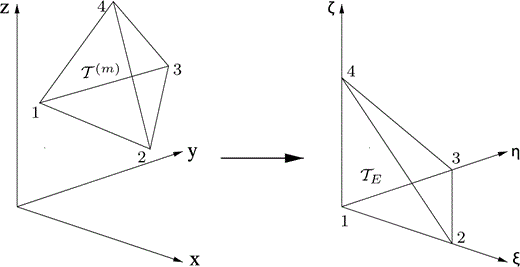
\includegraphics[width=0.6\linewidth]{figures/m_167-1-319-fig001.png}
    \caption{Transforming tetrahedron into a reference frame.(Figure taken from Figure 1 in ~\parencite{dumbser1})}
    \label{fig:transformation}
\end{figure}
As we are dealing with a new transformed coordinate system, we would need a Transformation matrix to transform the vector $Q_p$
from the global Cartesian system to the vector $Q_q^n$ in the normal, face-aligned frame. The transformation would be of the form

\begin{equation}
    Q_p = T_{pq}Q_q^n .
\end{equation}

\parencite{dumbser1} calculates the transformation matrix $T_{pq}$ as

\begin{align}
    \begin{split}
    T_{pq} = 
        \begin{bmatrix}
        n_x^2 & s_x^2 & t_x^2 & 2n_x s_x & 2s_x t_x & 2n_x t_x & 0 & 0 & 0 \\
        n_y^2 & s_y^2 & t_y^2 & 2n_y s_y & 2s_y t_y & 2n_y t_y & 0 & 0 & 0 \\
        n_z^2 & s_z^2 & t_z^2 & 2n_z s_z & 2s_z t_z & 2n_z t_z & 0 & 0 & 0 \\
        n_y n_x & s_y s_x & t_y t_x & n_y s_x + n_x s_y & s_y t_x + s_x t_y & n_y t_x + n_x t_y & 0 & 0 & 0 \\
        n_z n_y & s_z s_y & t_z t_y & n_z s_y + n_y s_z & s_z t_y + s_y t_z & n_z t_y + n_y t_z & 0 & 0 & 0 \\
        n_z n_x & s_z s_x & t_z t_x & n_z s_x + n_x s_z & s_z t_x + s_x t_z & n_z t_x + n_x t_z & 0 & 0 & 0 \\
        0 & 0 & 0 & 0 & 0 & 0 & n_x & s_x & t_x \\
        0 & 0 & 0 & 0 & 0 & 0 & n_y & s_y & t_y \\
        0 & 0 & 0 & 0 & 0 & 0 & n_z & s_z & t_z \\
    \end{bmatrix},
    \end{split}
\end{align}
where $\mathbf{n} = \left(n_x, n_y, n_z\right)^T$ are the components of the normal vector, and $\mathbf{s} = \left(s_x, s_y, s_z\right)^T$ and
$\mathbf{t} = \left(t_x, t_y, t_z\right)^T$ are the tangential vectors of the boundary face of the tetrahedron. $\mathbf{n}, \mathbf{s}, \mathbf{t}$
are orthogonal to each other. To represent the numerical solution $Q_h$ as a linear combination of pure spatial and pure time dependent functions, we introduce
the time-dependent degrees of freedom $\hat{Q}_m\left(t\right)$.

\begin{equation}
    Q_p^{\left(m\right)} \left(x,y,z,t\right) = \hat{Q}_{pl}^{\left(m\right)} \left(t\right) \Psi_l \left(x, y, z\right),
    \label{eq:mapping}
\end{equation}
where $\Psi_l\left(x,y,z\right)$ are spatial polynomial basis functions defined on the physical element. As it is more practical to define the polynomial 
basis functions on the reference element so that we can pre-calculate the integrals, we express equation \ref{eq:mapping} in 
the frame of the reference element using a suitable coordinate transformation M which maps the physical coordinates $\left(x, y, z\right)$ with the reference element $\left(\xi, \eta, \zeta\right)$

\begin{equation}
     Q_p^{\left(m\right)}\left(x,y,z,t\right) = \hat{Q}_{pl}^{\left(m\right)}\left(t\right) \Psi_l\left(M\left(x, y, z\right)\right).
\end{equation}

This formulation allows us to define the polynomial basis functions on the reference element $\Phi_l\left(\xi, \eta, \zeta\right)$.
As we can compute the integrals in the reference system beforehand, the coordinate transformation makes our implementation more computationally
efficient. This allows us to express $Q_h$ in each tetrahedron after the transformation of the coordinates
as 

\begin{equation}
    \left[Q_H^{\left(m\right)}\right]_p \left(\xi, \eta, \zeta, t\right) = \hat{Q}_{pl}^m \left(t\right) \Phi_l \left(\xi, \eta. \zeta\right),
\label{eq:solution}
\end{equation}
where $l$ denotes the $l^{th}$ basis function. Multiplying equation \ref{eq:compactform} with the test function $\Phi_k$ ~\parencite{cockburn2011discontinuous}
and integrating over our tetrahedral element $\mathcal{T}^{\left(m\right)}$ gives

\begin{equation}
    \int_{\mathcal{T}^{\left(m\right)}} \Phi_k \frac{\partial Q_p}{\partial t} dV + \int_{\mathcal{T}^{\left(m\right)}} \Phi_k \left(A_{pq} 
    \frac{\partial Q_q}{\partial x} + B_{pq}\frac{\partial Q_q}{\partial y} + C_{pq}\frac{\partial Q_q}{\partial z}\right)dV = 0.
    \label{eq:preweakformulation}
\end{equation}

We add fluxes $F_p^h$ at the boundaries of the tetrahedron to equation \ref{eq:preweakformulation} to include discontinuities in $Q_h$ and we integrate by parts to obtain the weak form as

\begin{equation}
    \int_{\mathcal{T}^{\left(m\right)}} \Phi_k \frac{\partial Q_p}{\partial t} dV + \int_{\partial \mathcal{T}^{\left(m\right)}} F_p^h dS
    - \int_{\mathcal{T}^{\left(m\right)}} \left(\frac{\partial \Phi_k}{\partial x} A_{pq}Q_q + \frac{\partial \Phi_k}{\partial y}B_{pq}Q_q
    + \frac{\partial \Phi_k}{\partial z}C_{pq}Q_q\right) dV = 0.
\label{eq:weakformulation}
\end{equation}

The flux between the tetrahedron $\mathcal{T}^{\left(m\right)}$ with the boundary extrapolated numerical solution $\hat{Q}_{sl} \Phi_l^{\left(m\right)}$
and one of its neighboring tetrahedra $\mathcal{T}^{\left(m_j\right)} \left(j=1,2,3,4\right)$ is computed in the global, coordinate system using the flux
matrix $A_{pq}$ from equation \ref{eq:fluxmatrix}

    \begin{align}
        \begin{split}
            F_p^h &= \frac{1}{2} T_{pq} \left(A_{qr}^{\left(m\right)} + \left|A_{qr}^{\left(m\right)}\right|\right)\left(T_{rs}\right)^{-1}
            \hat{Q}_{sl}^{\left(m\right)} \Phi_l^{\left(m\right)} \\
            &+ \frac{1}{2}T_{pq}\left(A_{qr}^{\left(m\right)} - \left|A_{qr}^{\left(m\right)}\right|\right)
            \left(T_{rs}\right)^{-1}\hat{Q}_{sl}^{\left(m_j\right)}\Phi_l^{\left(m_j\right)},            
        \end{split}
        \label{eq:fluxcalculation}
    \end{align}
where

\begin{equation}
\left|A_{qr}^{\left(m\right)}\right| = R_{qp}^A \left|\Lambda_{ps}\right| \left(R_{sr}\right)^{-1},
\end{equation}
and $\Lambda$ is the diagonal matrix with eigenvalues of $A_{pq}$ and $R_{pq}$ with right eigenvectors of $A_{pq}$ stacked in columns.
The next step would be inserting fluxes from equation \ref{eq:fluxcalculation} and $Q_h$ from equation \ref{eq:solution} into the weak
formulation in equation \ref{eq:weakformulation}. But as the basis functions $\Phi_l$ are defined in $\left(\xi, \eta, \zeta\right)$, we need
to transform the resulting equation with the transformation
\begin{equation}
    \text{d}x\, \text{d}y \, \text{d}z = \left|J\right| \text{d}\xi \,\text{d}\eta \,\text{d}\zeta,
\end{equation}
where $\left|J\right|$ is the determinant of the Jacobian matrix of the coordinate transformation and linear combination of the flux matrices to create transformed flux matrices
\begin{align}
    \begin{split}
        A_{pq}^{*} &= A_{pq} \frac{\partial \xi}{\partial x} + B_{pq} \frac{\partial \xi}{\partial y} + C_{pq} \frac{\partial \xi}{\partial z}, \\
        B_{pq}^{*} &= A_{pq} \frac{\partial \eta}{\partial x} + B_{pq} \frac{\partial \eta}{\partial y} + C_{pq} \frac{\partial \eta}{\partial z}, \\ 
        C_{pq}^{*} &= A_{pq} \frac{\partial \zeta}{\partial x} + B_{pq} \frac{\partial \zeta}{\partial y} + C_{pq} \frac{\partial \zeta}{\partial z}. 
    \end{split}
\end{align}

We finally get the semi-discrete \ac{DG} formulation of the ODE system within the reference tetrahedron $\mathcal{T}_E$
\begin{align}
    \begin{split}
        & \frac{\partial \hat{Q}_{pl}^{\left(m\right)}}{\partial t} \left|J\right| \int_{\mathcal{T}_E} \Phi_k \Phi_l d\xi d\eta d\zeta \\
        & + \sum_{j=1}^4 T_{pq}^j \frac{1}{2} \left(A_{qr}^{\left(m\right)} + \left| A_{qr}^{\left(m\right)}\right| \right) \left(T_{rs}^j\right)^{-1} \hat{Q}_{sl}^{\left(m\right)} \left|S_j\right| F_{kl}^{-,j} \\
        & + \sum_{j=1}^4 T_{pq}^j \frac{1}{2} \left(A_{qr}^{\left(m\right)} - \left| A_{qr}^{\left(m\right)}\right| \right) \left(T_{rs}^j\right)^{-1} \hat{Q}_{sl}^{\left(m_j\right)}\left|S_j\right| F_{kl}^{+,j,i,h} \\ 
        & - A_{pq}^* \hat{Q}_{ql}^{\left(m\right)} \left|J\right| \int_{\mathcal{T}_E} \frac{\partial \Phi_k}{\partial \xi} \Phi_l d\xi d\eta d\zeta \\
        & - B_{pq}^* \hat{Q}_{ql}^{\left(m\right)} \left|J\right| \int_{\mathcal{T}_E} \frac{\partial \Phi_k}{\partial \eta} \Phi_l d\xi d\eta d\zeta \\
        & - C_{pq}^* \hat{Q}_{ql}^{\left(m\right)} \left|J\right| \int_{\mathcal{T}_E} \frac{\partial \Phi_k}{\partial \zeta} \Phi_l d\xi d\eta d\zeta = 0,
    \end{split}
    \label{eq:finalform}
\end{align}
where 
\begin{align}
    \begin{split}
        F_{kl}^{-,j} &= \int_{\partial \left(\mathcal{T}_E\right)_j} \Phi_k \left(\xi^{\left(j\right)}\left(\chi, \tau\right)\right)\Phi_l \left(\xi^{\left(j\right)}\left(\chi, \tau\right)\right) d\chi d\tau, \quad \forall 1 \leq j\leq4 , \\
        F_{kl}^{+,j,i,h} &= \int_{\partial \left(\mathcal{T}_E\right)_j} \Phi_k \left(\xi^{\left(j\right)}\left(\chi, \tau\right)\right)\Phi_l \left(\xi^{\left(i\right)} \left( \tilde{\chi}^{(h)}\left(\chi, \tau\right), \tilde{\tau}^{\left(h\right)}\left(\chi, \tau\right) \right)\right) d\chi d\tau, \quad \forall 1 \leq i \leq 4, \quad 1 \leq h \leq 3.
    \end{split}
\end{align}

$F_{kl}^{-,j}$ accounts for the contribution of the element$\left(m\right)$ itself to the fluxes over face j and
$F_{kl}^{+,j,i,h}$ accounts for the contribution
of the element's direct side neighbor$\left(k_j\right)$ to the fluxes over the face $j$ and $\left|S_j\right|$ is the area of the face $j$ of the tetrahedron ~\parencite{dumbser1}. \\

\par We have not considered the source terms in the final formulation given in equation \ref{eq:finalform}. The source terms are dealt with as presented in~\parencite{10.1785/0120060253}.

\subsection[ADER Time Discretization]{ADER Time Discretization}

Instead of now utilizing the Runge-Kutta method to derive a limited fourth-order in time Runge-Kutta \ac{DG} scheme, we adopt the 
\ac{ADER} approach to achieve an arbitrary high-order accuracy in both spatial and temporal dimensions. Runge-Kutta schemes of order
higher than 4 tend to become inefficient as the number of calculation steps required exceeds the order of accuracy due to the Butcher barriers~\parencite{butcher1987numerical}.

\par By applying the \ac{ADER} scheme to the \ac{DG} formulation described in equation \ref{eq:finalform}, we obtain the \ac{ADER}-\ac{DG} scheme.
The crucial step in this approach involves using the Cauchy-Kovalewski procedure to replace time-derivatives with pure space derivatives.
As a consequence, the Cauchy-Kovalewski procedure provides the $k^{th}$ time-derivative as shown in equation \ref{eq:cauchy-kovalewski} in the face-aligned coordinate system, allowing us to
achieve higher accuracy without the limitations of tradiational Runge-Kutta schemes

\begin{equation}
    \frac{\partial^k Q_p}{\partial t^k} = \left(-1\right)^k \left(A_{pq}^* \frac{\partial}{\partial \xi} + B_{pq}^* \frac{\partial}{\partial \eta} + C_{pq}^* \frac{\partial}{\partial \zeta}\right)^k Q_q .
    \label{eq:cauchy-kovalewski}
\end{equation}

$Q_p$ can be expanded in a Taylor series with respect to time, and then the time derivatives can be substituted with space derivatives
using the equation \ref{eq:cauchy-kovalewski}~\parencite[Sec. 3.2]{dumbser1}. By adopting this approach, we can achieve arbitrary high-order
accuracy in both spatial and temporal dimensions. As previously mentioned, the \ac{ADER}-\ac{DG} schemes conduct time integration
within a single time step, considering only the current element and its neighboring elements, making it well-suited for parallelization.
Moreover, studies have demonstrated that the \ac{ADER}-\ac{DG} method outperforms traditional schemes such as \ac{RK-DG} scheme ~\parencite{dumbser2005ader}.
\subsection{Boundary Conditions}
Up until now, we have explored the time-discretization and space-discretization aspects of our problem. To complete our numerical
solver, we must establish suitable boundary conditions for the problem. We mainly have three kinds of boundaries in consideration.
\subsubsection{Absorbing Boundaries}
With the implementation of absorbing boundary conditions, the physical volume is enclosed by such boundaries in the forward direction. This means that no waves enter the computational domain, and any outgoing waves smoothly pass through the boundary without experiencing
reflection. A careful examination of equation \ref{eq:fluxcalculation} reveals that its first term on the right-hand side corresponds
to the outflow from the current element, while the second term represents the inflow from neighboring elements. To prevent incoming
waves from affecting the solution, we set the second term to zero. Consequently, the flux at all absorbing faces of the respective
tetrahedral elements is then appropriately set to

\begin{equation}
    F_p^{AbsorbBC} = \frac{1}{2} T_{pq} \left(A_{qr}^{\left(m\right)} + \left|A_{qr}^{\left(m\right)}\right|\right) \left(T_{rs}\right)^{-1} \hat{Q}_{sl}^{\left(m\right)} \Phi_l^{\left(m\right)}.
\end{equation}

\subsubsection{Free-Surface Boundaries}
At a free-surface boundary, the elastic medium is in contact with the surrounding air or void. In this scenario, there are no external forces
acting on the outside of the elastic medium. To ensure that normal and shear stresses vanish at the free surface, a technique involving
ghost cells is employed. These ghost cells are used to mirror the stresses, such that their values have the same magnitude as the actual
stresses but with the opposite sign. This approach effectively satisfies the condition of stress equilibrium at the free surface, allowing
for an accurate treatment at the boundary. We implement this using the flux function ~\parencite{dumbser1}

\begin{align}
    \begin{split}
    F_{p}^{FreeBC} &= \frac{1}{2}T_{pq}\left(A_{qr}^{\left(m\right)} + \left|A_{qr}^{\left(m\right)}\right|\right) \left(T_{rs}\right)^{-1} \hat{Q}_{sl}^{\left(m\right)} \Phi_l^{\left(m\right)}
    \\ &+ \frac{1}{2} T_{pq} \left(A_{qr}^{\left(m\right)} - \left|A_{qr}^{\left(m\right)}\right|\right) \Gamma_{rs} \left(T_{st}\right)^{-1} \hat{Q}_{tl}^{\left(m\right)} \Phi_l^{\left(m\right)} ,
    \end{split}
\end{align}
where $\Gamma_{rs} = diag\left(-1,1,1,-1,1,-1,1,1,1\right)$ is the matrix which mirrors the normal and shear stresses.

\section{Summary}
In this chapter we have discussed the governing equations of linear elasticity as a sytem of hyperbolic \ac{PDE}s. We then discussed the 
\ac{ADER}-\ac{DG} method for numerically solving this system of equations. We have also looked at the boundary conditions that we will use in our numerical solver.

% !TeX root = ../main.tex
% Add the above to each chapter to make compiling the PDF easier in some editors.

\chapter{\ac{ITM} on a 1D Acoustic Planar Wave}\label{chapter:ITMAcoustic}
In this chapter, we calculate the analytical solution for a 1D Acoustic wave when an \ac{ITM} is applied from $t_{ITM}^-$ to $t_{ITM}^+$.
For this, we consider a 1D Acoustic Equation [~\parencite[Sec. 2.8]{leveque_2002}] linearized about the motionless state:
\begin{align}
    \begin{split}
        p_t + K_0u_x = 0, \\
        u_t + \frac{1}{\rho_0}p_x = 0 .\\
    \end{split}
\end{align}

where $p$ is the pressure perturbation, $K_0$ is the bulk modulus of the material and $u$ is the velocity purturbation. 
This can be written in consolidated matrix vector form as done for first order hyperbolic systems of equations as follows:

\begin{align}
    \begin{split}
    \begin{bmatrix}
        p \\
        u
    \end{bmatrix}_t + 
    \begin{bmatrix}
        0 & K_0 \\
        \frac{1}{\rho_0} & 0 \\
    \end{bmatrix}
    \begin{bmatrix}
        p \\
        u
    \end{bmatrix}_x = 0
    \end{split}
    \label{eq:acoustic}
\end{align}.

The flux matrix for equation \ref{eq:acoustic} has two eigenvalues:

\begin{align}
    \begin{split}
        \lambda_1 = -c_0; \lambda_2 = c_0,
    \end{split}
\end{align}

where 
\begin{align}
    \begin{split}
        c_0 = \sqrt{\frac{K_0}{\rho_0}}
    \end{split}
\end{align}

which is the speed of sound in gas. And waves can propagate in either direction with this speed. The eigenvectors for this coefficient matrix come out to be:

\begin{align}
    \begin{split}
        r^1 = \begin{bmatrix}
            -\rho_0 c_0 \\
            1
        \end{bmatrix}, 
        r^2 = \begin{bmatrix}
            \rho_0 c_0 \\
            1
        \end{bmatrix}.
    \end{split}
\end{align}

The impedance is defined as:
\begin{equation}
    Z_0 = \rho_0 c_0.
\end{equation}.

Using these parameters, ~\parencite[Sec. 2.8]{leveque_2002} calculates the solution of the acoustic equation depending on the initial conditions $p^0(x), u^0(x)$ as:
\begin{align}
    \begin{split}
        p(x,t) &= \frac{1}{2}\left[p^0\left(x + c_0t\right) + p^0\left(x - c_0t\right)\right] - \frac{Z_0}{2}\left[u^0\left(x+c_0t\right) - u^0\left(x-c_0t\right)\right], \\
        u(x,t) &= -\frac{1}{2Z_0}\left[p^0\left(x+c_0t\right) - p^0\left(x-c_0t\right)\right] + \frac{1}{2}\left[u^0\left(x+c_0t\right) + u^0\left(x-c_0t\right)\right] .
    \end{split}
    \label{eq:solutionacoustic}
\end{align}

We use this solution to find the analytical solution of a 1D acoustic wave after the \ac{ITM} is applied in two different ways. First we ensure we use initial conditions which give rise to only one forward wave. We simply use a sinusoidal wave multiplied to only one eigenvector $r^2$.
This defines our initial conditions as
\begin{align}
    \begin{split}
        p^0\left(x\right) &= \rho_0c_0cos\left(kx\right), \\
        u^0\left(x\right) &= cos\left(kx\right)
    \end{split}
    \label{eq:initialconditions}
\end{align}

where $k$ is the wave number of the wave. The energy of the system is defined as (~\parencite{Kopriva2021}):

\begin{align}
    \begin{split}
     E_1 &= \int_{-\frac{\pi}{k}}^{\frac{\pi}{k}} \left(\frac{1}{2K}p^2 + \frac{1}{2}\rho u^2\right) dx , \\
     \implies E_1 &= \frac{\pi\rho_0}{k} .
    \end{split}
    \label{eq:energy}
\end{align}

\section{Impedance Changing \ac{ITM}}\label{section:impedanceconstantITM}
Using the conditions given in equation \ref{eq:initialconditions}, we calculate the solution at $t_ITM^-$ and use them as initial conditions for the new equation where the wave velocities are scaled.
In this case, we scale the velocities such that the impedance also changes(keeping the density constant). Using \ref{eq:solutionacoustic}, we get the initial conditions for the next phase of the simulation$\left(t_{ITM}^- \leq t \leq t_{ITM}^+ \right)$ at $t_{ITM}^-$ as:

\begin{align}
    \begin{split}
        p^0_{t_{ITM}^-}\left(x\right) &= c_0 \rho_0 cos\left(kx - c_0kt_{ITM}^-\right), \\
        u^0_{t_{ITM}^-}\left(x\right) &= cos\left(kx - c_0kt_{ITM}^-\right) .
    \end{split}
\end{align}

We now use these as the initial conditions and equation \ref{eq:solutionacoustic} with the updated wave velocity and constant density to get the evolved solution for $t_{ITM}^- \leq t \leq t_{ITM}^+ $. ~\parencite{sagemath} was used to perform the simplifications for the arithmetic. We obtain the solution for this period as:

\begin{align}
    \begin{split}
        p_{2}\left(x, t\right) &= -\frac{1}{2} \left(n-1\right)c_0\rho_0cos\left(kx + c_0knt - \left(c_0kn + c_0k\right)t_{ITM}^-\right) \\
        &+ \frac{1}{2} \left(n+1\right)c_0\rho_0cos\left(kx - c_0knt + \left(c_0kn - c_0k\right)t_{ITM}^-\right), \\
        u_{2}\left(x, t\right) &= \frac{1}{2}\left(n-1\right)cos\left(kx + c_0knt - \left(c_0kn + c_0k\right)t_{ITM}^-\right)\\
        &+ \frac{1}{2}\left(n+1\right)cos\left(kx - c_0knt + \left(c_0kn-c_0k\right)t_{ITM^-}\right)
    \end{split}
\end{align}

where n is the velocity scaling factor. We now use these expressions to calculate the energy as we have already done in equation \ref{eq:energy}. This gives us the energy in second phase i.e., $t_{ITM}^- \leq t \leq t_{ITM}^+ $ to be:
\begin{equation}
    E_2 = \frac{1}{2}\frac{\left(1 + n^2\right)\pi \rho_0}{kn^2} .
\end{equation}

This shows that the energy drops when the velocity is scaled up. We then check the relative drop in energy for different scaling factors and see that it asymptotes to 0.5 for higher scaling factors. The variation of the ratio with the scaling factor can be seen in figure \ref{fig:ratio1}.

\begin{figure}
    \centering
    \begin{tikzpicture}[scale=1.0]
        \begin{axis}[
            ylabel = $\frac{E_2}{E_1}$,
            xlabel = $n$]
            \addplot[domain=0:10, black, ultra thick]{0.5*(1+x*x)/(x*x)};
        \end{axis}
    \end{tikzpicture}
    \caption{Relative Energy in $t_{ITM}^- \leq t \leq t_{ITM}^+$}
    \label{fig:ratio1}
\end{figure}

Now the velocity is scaled down again to its original value at $t=t_{ITM}^+$ and defining $\tau = t_{ITM}^+ - t_{ITM}^-$, we do a similar calculation to obtain the solution for the final phase: $t \geq t_{ITM}^+$ and the solution as:

\begin{align}
    \begin{split}
        p_3\left(x, t\right) & = -\frac{{\frac{1}{4}c_{0}\rho_{0}\left( n^{2} + 1\right)} \cos\left(k x + c_{0} k t - 2 \, c_{0} k \mathit{t_{ITM}^-} - {\left(c_{0} k n + c_{0} k\right)} \tau\right)}{n} \\
        & - \frac{{\frac{1}{4}c_0\rho_0\left(n^{2} - 1\right)} \cos\left(k x + c_{0} k t - 2 \, c_{0} k \mathit{t_{ITM}^-} + {\left(c_{0} k n - c_{0} k\right)} \tau\right)}{n} \\
        & - \frac{{\frac{1}{4}c_0\rho_0\left(n^{2} - 2n + 1\right)} \cos\left(kx -c_{0} k t + {\left(c_{0} k n + c_{0} k\right)} \tau\right)}{n} \\
        & - \frac{{\frac{1}{4}c_0\rho_0\left(-n^{2} - 2n - 1\right)} \cos\left(kx-c_{0} k t - {\left(c_{0} k n - c_{0} k\right)} \tau\right)}{n}, \\
        u_3\left(x, t\right) & =  -\frac{{\frac{1}{4}\left(n^{2} - 1\right)} \cos\left( k x + c_{0} k t - 2 \, c_{0} k \mathit{t_{ITM}^-} - {\left(c_{0} k n + c_{0} k\right)} \tau\right)}{n} \\
        & - \frac{{\frac{1}{4}\left(-n^{2} + 1\right)} \cos\left(kx + c_{0} k t - 2 \, c_{0} k \mathit{t_{ITM}^-} + {\left(c_{0} k n - c_{0} k\right)} \tau\right)}{n} \\
        & - \frac{{\frac{1}{4}\left(n^{2} - 2n + 1\right)} \cos\left(kx -c_{0} k t + {\left(c_{0} k n + c_{0} k\right)} \tau\right)}{n} \\
        & - \frac{{\frac{1}{4}\left(-n^{2} - 2n - 1\right)} \cos\left(kx -c_{0} k t - {\left(c_{0} k n - c_{0} k\right)} \tau\right)}{n} .
    \end{split}
\end{align}

Using these quantities, we now calculate the energy using the equation \ref{eq:energy}
\begin{equation}
    E_3 = -\pi \rho_0\frac{{\left(1 + n^{4} - 2 \, n^{2}\right)} \cos^{2}\left(c_{0} k n \tau\right) - {\left(1 + n^{4}\right)}}{2 \, k n^{2}}.
\end{equation}

We observe that this ratio is dependent on the parameters: $k, n, \tau$ and is bounded as

\begin{equation}
    \frac{\pi \rho_0}{K} \leq E_3 \leq \frac{\pi \rho_0}{2K}\left[n^2 + \frac{1}{n^2}\right]
\end{equation}

We compare the worst case scenario i.e., what would be the maximum energy increase after the ITM is applied. For that we take the upper bound and plot that function with $n$ as we did before in figure \ref{fig:ratio2}.

\begin{figure}
    \centering
    \begin{tikzpicture}[scale=1.0]
        \begin{axis}[
            ylabel = $\frac{E_3}{E_1}$,
            xlabel = $n$]
            \addplot[domain=0.1:10, black, ultra thick]{0.5*((1/x)^2 + x^2)};
        \end{axis}
    \end{tikzpicture}
    \caption{Relative Energy in $t \geq t_{ITM}^+$}
    \label{fig:ratio2}
\end{figure}

The minimum value for this energy jump lies at $n=1$ which means no velocity scaling and no reflections. This case is of no use to us.

\section{Constant Impedance \ac{ITM}}
We know that there is no reflected wave in space interfaces when the impedance stays constant. Here, we test out the same with a time interface i.e., we perform \ac{ITM} such that the velocities scale but the impedance stays constant. This is achieved by scaling the wave speed by $n$ and the density by $\frac{1}{n}$.
Similar to section \ref{section:impedanceconstantITM}, we choose the initial conditions as

\begin{align}
    \begin{split}
        p^0\left(x\right) &= Z_0cos\left(kx\right), \\
        u^0\left(x\right) &= cos\left(kx\right) .
    \end{split}
    \label{eq:initialconditions2}
\end{align}

Using these parameters, the energy is once again computed as

\begin{equation}
    E_1 = \frac{\pi Z_0}{c_0 k}
\end{equation}

Using the conditions given in equation \ref{eq:initialconditions2}, we calculate the solution at $t_ITM^-$ and use them as initial conditions for the new equation where the wave velocities are scaled.
In this case, we scale the velocities such that the impedance does not change(density is scaled down). Using \ref{eq:solutionacoustic}, we get the initial conditions for the next phase of the simulation$\left(t_{ITM}^- \leq t \leq t_{ITM}^+ \right)$ at $t_{ITM}^-$ as

\begin{align}
    \begin{split}
        p^0_{t_{ITM}^-}\left(x\right) &= Z_0 cos\left(kx - c_0kt_{ITM}^-\right), \\
        u^0_{t_{ITM}^-}\left(x\right) &= cos\left(kx - c_0kt_{ITM}^-\right) .
    \end{split}
\end{align}

We now use these as the initial conditions and equation \ref{eq:solutionacoustic} with the updated wave velocity and constant density to get the evolved solution for $t_{ITM}^- \leq t \leq t_{ITM}^+ $. ~\parencite{sagemath} was used to perform the simplifications for the arithmetic. We obtain the solution for this period as:

\begin{align}
    \begin{split}
        p_{2}\left(x, t\right) &= Z_{0} \cos\left(kx -c_{0} k n t + {\left(c_{0} k n - c_{0} k\right)} \mathit{t_{ITM}^-}\right), \\
        u_{2}\left(x, t\right) &= \cos\left(kx -c_{0} k n t + {\left(c_{0} k n - c_{0} k\right)} \mathit{t_{ITM}^-} \right)
    \end{split}
\end{align}

where n is the velocity scaling factor. We now use these expressions to calculate the energy as we have already done in equation \ref{eq:energy}. This gives us the energy in second phase i.e., $t_{ITM}^- \leq t \leq t_{ITM}^+ $ to be:
\begin{equation}
    E_2 = \frac{\pi z_{0}}{c_{0} k n} .
\end{equation}

Two interesting observations that can be made here are that:
\begin{enumerate}
    \item There is no extra reflected wave and the wave speed is just increased with a phase shift
    \item The energy is directly scaled down by the velocity scaling factor
\end{enumerate}

% \begin{figure}
%     \centering
%     \begin{tikzpicture}[scale=1.0]
%         \begin{axis}[
%             ylabel = $\frac{E_2}{E_1}$,
%             xlabel = $n$]
%             \addplot[domain=0:10, black, ultra thick]{0.5*(1+x*x)/(x*x)};
%         \end{axis}
%     \end{tikzpicture}
%     \caption{Relative Energy in $t_{ITM}^- \leq t \leq t_{ITM}^+$}
%     \label{fig:ratio1}
% \end{figure}

Now the velocity is scaled down again to its original value at $t=t_{ITM}^+$ and defining $\tau = t_{ITM}^+ - t_{ITM}^-$, we do a similar calculation to obtain the solution for the final phase: $t \geq t_{ITM}^+$ and the solution as:

\begin{align}
    \begin{split}
        p_3\left(x, t\right) & = Z_{0} \cos\left(kx - c_{0} k t - {\left(c_{0} k n - c_{0} k\right)} \tau\right)\\
        u_3\left(x, t\right) & =  \cos\left(kx - c_{0} k t - {\left(c_{0} k n - c_{0} k\right)} \tau\right)
    \end{split}
\end{align}

Using these quantities, we now calculate the energy using the equation \ref{eq:energy}
\begin{equation}
    E_3 = \frac{\pi Z_0}{c_0 k}
\end{equation}

which is equal to $E_1$. This shows that there is no final energy increase when the impedance is kept constant. The final solution also has no reflected wave and has the same wave speed as the initial wave and has a phase shift in time. This confirms that even in time interfaces, similar to space interfaces there is no reflection.

% \begin{align}
%     \begin{split}
%         \left(\left(\begin{array}{rrrr}
%             1 & 1 & 0 & 0 \\
%             -\frac{k_{1}}{\rho_{0} \sqrt{\frac{K_{0} k_{1}^{2} + K_{0} k_{2}^{2} + K_{0} k_{3}^{2}}{\rho_{0}}}} & \frac{k_{1}}{\rho_{0} \sqrt{\frac{K_{0} k_{1}^{2} + K_{0} k_{2}^{2} + K_{0} k_{3}^{2}}{\rho_{0}}}} & 1 & 0 \\
%             -\frac{k_{2}}{\rho_{0} \sqrt{\frac{K_{0} k_{1}^{2} + K_{0} k_{2}^{2} + K_{0} k_{3}^{2}}{\rho_{0}}}} & \frac{k_{2}}{\rho_{0} \sqrt{\frac{K_{0} k_{1}^{2} + K_{0} k_{2}^{2} + K_{0} k_{3}^{2}}{\rho_{0}}}} & 0 & 1 \\
%             -\frac{k_{3}}{\rho_{0} \sqrt{\frac{K_{0} k_{1}^{2} + K_{0} k_{2}^{2} + K_{0} k_{3}^{2}}{\rho_{0}}}} & \frac{k_{3}}{\rho_{0} \sqrt{\frac{K_{0} k_{1}^{2} + K_{0} k_{2}^{2} + K_{0} k_{3}^{2}}{\rho_{0}}}} & -\frac{k_{1}}{k_{3}} & -\frac{k_{2}}{k_{3}}
%             \end{array}\right)\right)
%     \end{split}
% \end{align}

\chapter{\ac{ITM} on a 3D Acoustic Planar Wave}\label{chapter:3DITMAcoustic}
In this chapter, we calculate the analytical solution for a 3D Acoustic wave when an \ac{ITM} is applied from $t_{ITM}^-$ to $t_{ITM}^+$.

For this, we consider a 3D Acoustic Equation linearized about the motionless state:

where $p$ is the pressure perturbation, $K_0$ is the bulk modulus of the material and $u$ is the velocity purturbation. 
This can be written in consolidated matrix vector form as done for first order hyperbolic systems of equations as follows:

\begin{align}
    \begin{split}
        \mathbf{q_t} + \mathbf{Aq_x} + \mathbf{Bq_y} + \mathbf{Cq_z} = 0,
    \end{split}
    \label{eq:3Dacoustic}
\end{align}

where 

\begin{align}
    \begin{split}
        \mathbf{q} = \begin{bmatrix}
            p \\
            u \\
            v
        \end{bmatrix},
        \mathbf{A} = \begin{bmatrix}
            0 & K_0 & 0 & 0 \\
            \frac{1}{\rho_0} & 0 & 0 & 0 \\
            0 & 0 & 0 & 0 \\
            0 & 0 & 0 & 0 \\
        \end{bmatrix},
        \mathbf{B} = \begin{bmatrix}
            0 & 0 & K_0 & 0 \\
            0 & 0 & 0 & 0 \\
            \frac{1}{\rho_0} & 0 & 0 & 0 \\
            0 & 0 & 0 & 0 \\
        \end{bmatrix},
        \mathbf{C} = \begin{bmatrix}
            0 & 0 & 0 & K_0 \\
            0 & 0 & 0 & 0 \\
            0 & 0 & 0 & 0 \\
            \frac{1}{\rho_0} & 0 & 0 & 0 \\
        \end{bmatrix}.
    \end{split}
\end{align}

We assume an ansatz of 
\begin{equation}
    \mathbf{q}\left(\mathbf{x}, t\right) = \mathbf{q_0} cos\left(\mathbf{k}\cdot\mathbf{x} - \omega t\right),
\end{equation}

where $\mathbf{k}=\left(k_1, k_2, k_3\right)$ is the direction of the planar wave. Using the derivatives of equation \ref{eq:3Dacoustic},

\begin{align}
    \begin{split}
    \frac{\partial \mathbf{q}}{\partial t} = \omega \mathbf{q_0} sin\left(\mathbf{k}\cdot\mathbf{x} - \omega t\right),
    \frac{\partial \mathbf{q}}{\partial x} = -k_1 \mathbf{q_0} sin\left(\mathbf{k}\cdot\mathbf{x} - \omega t\right), \\
    \frac{\partial \mathbf{q}}{\partial y} = -k_2 \mathbf{q_0} sin\left(\mathbf{k}\cdot\mathbf{x} - \omega t\right),
    \frac{\partial \mathbf{q}}{\partial z} = -k_3 \mathbf{q_0} sin\left(\mathbf{k}\cdot\mathbf{x} - \omega t\right).
\end{split}
\end{align}

Substituting these back in the equation we get,

\begin{align}
    \begin{split}
        \left(\omega - \mathbf{A}k_1 - \mathbf{B}k_2 - \mathbf{C}k_3\right)\mathbf{q_0}sin\left(\mathbf{k}\cdot\mathbf{x} - \omega t\right) = 0.
    \end{split}
\end{align}

Dividing by $sin\left(\mathbf{k}\cdot\mathbf{x} - \omega t\right)$ and rearranging the terms, we get

\begin{align}
    \begin{split}
        \left(\mathbf{A}k_1 + \mathbf{B}k_2 + \mathbf{C}k_3\right)\mathbf{q_0} = \omega \mathbf{q_0}
    \end{split}
\end{align}

This shows that $\omega$ is an eigenvalue of $\mathbf{\hat{A}} = \mathbf{A}k_1 + \mathbf{B}k_2 + \mathbf{C}k_3$ and $\mathbf{q_0}$ is an eigenvector. The modified matrix $\mathbf{\hat{A}}$ would then be

\begin{align}
    \begin{split}
    \mathbf{\hat{A}} = \left(\begin{array}{rrrr}
0 & K_{0} k_{1} & K_{0} k_{2} & K_{0} k_{3} \\
\frac{k_{1}}{\rho_{0}} & 0 & 0 & 0 \\
\frac{k_{2}}{\rho_{0}} & 0 & 0 & 0 \\
\frac{k_{3}}{\rho_{0}} & 0 & 0 & 0
\end{array}\right)
    \end{split}
\end{align}

with the set of eigenvalues

\begin{align}
    \begin{split}
        \omega_1 = -\sqrt{\frac{K_{0} k_{1}^{2}}{\rho_{0}} + \frac{K_{0} k_{2}^{2}}{\rho_{0}} + \frac{K_{0} k_{3}^{2}}{\rho_{0}}},
        \omega_2 = 0,
        \omega_3 = 0,
        \omega_4 = \sqrt{\frac{K_{0} k_{1}^{2}}{\rho_{0}} + \frac{K_{0} k_{2}^{2}}{\rho_{0}} + \frac{K_{0} k_{3}^{2}}{\rho_{0}}};
    \end{split}
\end{align}

and the eigenvectors

\begin{align}
    \begin{split}
    \mathbf{r_1} = \begin{bmatrix}
        1 \\
-\frac{k_{1}}{\rho_{0} \sqrt{\frac{K_{0} k_{1}^{2} + K_{0} k_{2}^{2} + K_{0} k_{3}^{2}}{\rho_{0}}}} \\
-\frac{k_{2}}{\rho_{0} \sqrt{\frac{K_{0} k_{1}^{2} + K_{0} k_{2}^{2} + K_{0} k_{3}^{2}}{\rho_{0}}}} \\
-\frac{k_{3}}{\rho_{0} \sqrt{\frac{K_{0} k_{1}^{2} + K_{0} k_{2}^{2} + K_{0} k_{3}^{2}}{\rho_{0}}}}
        \end{bmatrix},
        \mathbf{r_2} = \begin{bmatrix}
            0 \\
1 \\
0 \\
-\frac{k_{1}}{k_{3}}
            \end{bmatrix},
            \mathbf{r_3} = \begin{bmatrix}
                0 \\
                0 \\
                1 \\
                -\frac{k_{2}}{k_{3}}
                \end{bmatrix},
                \mathbf{r_4} = \begin{bmatrix}
                    1 \\
\frac{k_{1}}{\rho_{0} \sqrt{\frac{K_{0} k_{1}^{2} + K_{0} k_{2}^{2} + K_{0} k_{3}^{2}}{\rho_{0}}}} \\
\frac{k_{2}}{\rho_{0} \sqrt{\frac{K_{0} k_{1}^{2} + K_{0} k_{2}^{2} + K_{0} k_{3}^{2}}{\rho_{0}}}} \\
\frac{k_{3}}{\rho_{0} \sqrt{\frac{K_{0} k_{1}^{2} + K_{0} k_{2}^{2} + K_{0} k_{3}^{2}}{\rho_{0}}}}
                    \end{bmatrix},
    \end{split}
\end{align} .

For the sake of simplicity to verify what happens in the case of ITM, we consider the initial condition to be along one eigenvector(here choosing $r_4$).
This makes our wave to be of the form 

\begin{align}
    \begin{split}
        \mathbf{q_1}\left(\mathbf{x}, t\right) = \begin{bmatrix}
            1 \\
\frac{k_{1}}{\rho_{0} \sqrt{\frac{K_{0} k_{1}^{2} + K_{0} k_{2}^{2} + K_{0} k_{3}^{2}}{\rho_{0}}}} \\
\frac{k_{2}}{\rho_{0} \sqrt{\frac{K_{0} k_{1}^{2} + K_{0} k_{2}^{2} + K_{0} k_{3}^{2}}{\rho_{0}}}} \\
\frac{k_{3}}{\rho_{0} \sqrt{\frac{K_{0} k_{1}^{2} + K_{0} k_{2}^{2} + K_{0} k_{3}^{2}}{\rho_{0}}}}
            \end{bmatrix} cos\left(\mathbf{k}\cdot\mathbf{x} - \sqrt{\frac{K_{0} k_{1}^{2}}{\rho_{0}} + \frac{K_{0} k_{2}^{2}}{\rho_{0}} + \frac{K_{0} k_{3}^{2}}{\rho_{0}}} t\right) .
    \end{split}
\end{align}
It can be verified that this wave form satifies our PDE in equation \ref{eq:3Dacoustic}.

Now, in phase 2 i.e., when ITM is applied, we get a modified $\mathbf{\hat{A}}$ as we change our material properties specifically $K_0$ to $n^2K_0$. The modified matrix would then be

\begin{align}
    \begin{split}
    \mathbf{\hat{A}_2} = \begin{bmatrix}
        0 & K_{0} k_{1} n^{2} & K_{0} k_{2} n^{2} & K_{0} k_{3} n^{2} \\
\frac{k_{1}}{\rho_{0}} & 0 & 0 & 0 \\
\frac{k_{2}}{\rho_{0}} & 0 & 0 & 0 \\
\frac{k_{3}}{\rho_{0}} & 0 & 0 & 0
    \end{bmatrix},
    \end{split}
\end{align}

with eigenvalues

\begin{align}
    \begin{split}
    \omega_1^2 = -n \sqrt{\frac{K_{0} k_{1}^{2}}{\rho_{0}} + \frac{K_{0} k_{2}^{2}}{\rho_{0}} + \frac{K_{0} k_{3}^{2}}{\rho_{0}}},
    \omega_2^2 = 0,
    \omega_3^2 = 0,
    \omega_4^2 = n \sqrt{\frac{K_{0} k_{1}^{2}}{\rho_{0}} + \frac{K_{0} k_{2}^{2}}{\rho_{0}} + \frac{K_{0} k_{3}^{2}}{\rho_{0}}},
    \end{split}
\end{align}

and eigenvectors

\begin{align}
    \begin{split}
    \mathbf{r_1^2} = \begin{bmatrix}
        1 \\
-\frac{k_{1}}{n \rho_{0} \sqrt{\frac{K_{0} k_{1}^{2} + K_{0} k_{2}^{2} + K_{0} k_{3}^{2}}{\rho_{0}}}} \\
-\frac{k_{2}}{n \rho_{0} \sqrt{\frac{K_{0} k_{1}^{2} + K_{0} k_{2}^{2} + K_{0} k_{3}^{2}}{\rho_{0}}}} \\
-\frac{k_{3}}{n \rho_{0} \sqrt{\frac{K_{0} k_{1}^{2} + K_{0} k_{2}^{2} + K_{0} k_{3}^{2}}{\rho_{0}}}}
        \end{bmatrix},
        \mathbf{r_2^2} = \begin{bmatrix}
            0 \\
            1 \\
            0 \\
            -\frac{k_{1}}{k_{3}}
            \end{bmatrix},
            \mathbf{r_3^2} = \begin{bmatrix}
                0 \\
0 \\
1 \\
-\frac{k_{2}}{k_{3}}
                \end{bmatrix},
                \mathbf{r_4^2} = \begin{bmatrix}
                    1 \\
                    \frac{k_{1}}{n \rho_{0} \sqrt{\frac{K_{0} k_{1}^{2} + K_{0} k_{2}^{2} + K_{0} k_{3}^{2}}{\rho_{0}}}} \\
                    \frac{k_{2}}{n \rho_{0} \sqrt{\frac{K_{0} k_{1}^{2} + K_{0} k_{2}^{2} + K_{0} k_{3}^{2}}{\rho_{0}}}} \\
                    \frac{k_{3}}{n \rho_{0} \sqrt{\frac{K_{0} k_{1}^{2} + K_{0} k_{2}^{2} + K_{0} k_{3}^{2}}{\rho_{0}}}}
                    \end{bmatrix},
    \end{split}
\end{align} .

Now as we expect two waves going in 2 opposite directions, we take weighted sum of the two directional waves and assume an ansatz that in phase 2 i.e., $t_{ITM}^- \leq t \leq t_{ITM}^+ $, we have the following wave form introducing some phase shift in both the waves:

\begin{align}
    \begin{split}
        \mathbf{q_2} \left(\mathbf{x}, t\right) = w_1 \mathbf{r_1^2} cos\left(\mathbf{k}\cdot\mathbf{x} -\omega_1^2 t + \phi_1\right) + w_2 \mathbf{r_4^2} cos\left(\mathbf{k}\cdot\mathbf{x} - \omega_4^2 t + \phi_2\right).
    \end{split}
    \end{align}

One can verify that this satsfies the PDE by substituting it in the PDE with the modified matrices. Now at $t=t_{ITM}^-$, the solution must be continuos for all space, i.e.,

\begin{align}
    \begin{split}
    \mathbf{q_1}\left(\mathbf{x}, t_{ITM}^-\right) = \mathbf{q_2}\left(\mathbf{x}, t_{ITM}^-\right)
    \end{split}
\end{align}

Solving for the required coefficients...
% TODO: add more chapters here

\appendix{}

\microtypesetup{protrusion=false}

\addchap{Abbreviations}
\begin{acronym}
	\itemsep-.25\baselineskip
	\acro{TUM}[TUM]{Technical University of Munich}
	\acro{ITM}[ITM]{Instantaneous Time Mirror}
	\acro{DG}[DG]{Discontinuous Galerkin}
	\acro{ADER}[ADER]{Arbitrary high-order schemes using DERivates}
	\acro{DG-FE}[DG-FE]{Discontinuous Galerkin Finite Element}
	\acro{RK-DG}[RK-DG]{Runge Kutta Discontinuous Galerkin}
	% TODO: add acronyms
\end{acronym}

\listoffigures{}
\listoftables{}
\microtypesetup{protrusion=true}
\printbibliography{}

\end{document}
